\chapter{Nodal Analysis}

\section{Basic Idea}
A circuit with $b$ branches has $2b$ unknowns since there are $b$ voltages and $b$ currents. Hence, $2b$ linear independent equations are required to solve the circuit. If the circuit has $n$ nodes and $b$ branches, it has
\begin{itemize}
 \item Kirchoff's current law (KCL) equations
 \item Kirchoff's voltage law (KVL) equations
 \item Characteristic equations (Ohm's Law in a broad sense.)
\end{itemize}  
There are only $n-1$ KCLs since the nth equation is a linear combination of the remaining $n-1$. At the same time, it can be demonstrated that if we can imagine a very high number of
closed paths in the network only $b-n+1$ are able to provide independent KVLs. Finally there are $b$ characteristic equations, describing the behavior of the branch, making a total of $2b$ linear independent equations.

To prove the number of independent KVLs equations, let us consider a generic electrical circuit. Let us now substitute the circuit with one oriented graph i.e. with a diagram composed of oriented arcs where each arc represents one of the branches of the original circuit.
With this substitution we can focus simply on the topology disregarding the characteristics of the specific branch. In effect our conclusion regarding the KVL must be valid for every network no matter the branches involved and then it makes sense to focus
only on the connections.

\begin{figure}[ht]
	\centering
	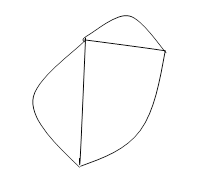
\includegraphics[scale=0.6]{img/graph_representation_1.png} 
	\caption{Graph representing the topology of an electrical circuit}
	\label{fig:graph_rep_1}
\end{figure}

Let us now orient the arc, exactly as we assume to assume a direction for the measurement of the current and let us also number the arcs.

\begin{figure}[ht]
	\centering
	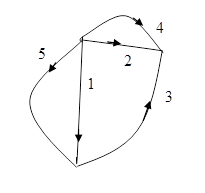
\includegraphics[scale=0.6]{img/graph_representation_2.png} 
	\caption{Oriented graph representing the topology of an electrical circuit}
	\label{fig:graph_rep_2}
\end{figure}

Let us now define a so called tree for this graph. A tree is given by a subset of arcs that connects all the nodes but do not create any closed path.

\begin{figure}[ht]
	\centering
	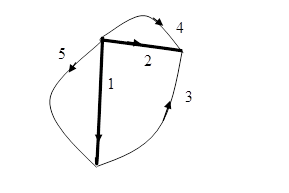
\includegraphics[scale=0.6]{img/graph_representation_3.png} 
	\caption{Selecting a tree of the graph}
	\label{fig:graph_rep_3}
\end{figure}

It is pretty easy to understand that to connect $n$ nodes without creating a closed path we are going to need $n-1$ arcs. As result $b-n+1$ arcs are not included in the tree (this is actually called co-tree).

For this network for example we have:
\begin{align}
\begin{split}
	b &= 5 \\
	n &= 3
\end{split}
\end{align}

So the tree includes 2 branches and the co-tree includes 3 branches.

\section{Basic Steps}
The nodal analysis method reduces the number of equations that need to be solved simultaneously. $n-1$ voltage variables are defined and solved, writing $n-1$ KCL based equations. 
A circuit can be solved using Nodal Analysis, by observing the following steps:

\begin{itemize}
\item Step 1: Select a reference node (mathematical ground) and number the remaining $n-1$ nodes, that are the independent voltage variables
\item Step 2: Represent every branch current $i$ as a function of node voltage variables $e$ with the general expression $i_k = g(e)$
\item Step 3: Write $n-1$ KCL based equations in terms of node voltage variable. The resulting equations can be written in matrix form and has to be solved for $e$.
\begin{equation} \label{eq:nodalAnalysis}
G_{n-1}e_{n-1} =  A_{n-1}
\end{equation}
\end{itemize}

\section{Matrix Stamp Concept}
The matrix stamp concept is an approach to construct the matrix equation \ref{eq:nodalAnalysis}. Each element of the circuit will stamp the matrix equation in certain position.

\subsection{Resistor} \label{ResistorMatrixStamp}
A resistor R between the nodes j and k will stamp the conductance matrix $G$ in the positions j,j and k,k with the value $\frac{1}{R} $ and in the positions j,k and k,j with the value $\frac{-1}{R} $.

\begin{align}
\begin{split}
&
\begin{matrix}
& \cdots & j & \quad k & \cdots
\end{matrix}\\[-5pt]
G \quad = \quad
\begin{matrix}
\vdots\\[6pt]
j\\[6pt]
k\\[6pt]
\vdots\\
\end{matrix}
&
\begin{bmatrix}
	\quad & \quad &  \\[6pt]
	\quad & \dfrac{1}{R} & \dfrac{-1}{R} & \quad  \\[6pt]
	\quad & \dfrac{-1}{R} & \dfrac{1}{R} & \quad \\[6pt]
	\quad &  & 
\end{bmatrix}
\end{split}
\end{align}

\begin{figure}[h]
	\centering
	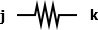
\includegraphics[scale=0.6]{img/Resistor.png}
	\caption{Resistor between nodes j and k}
	\label{fig:Resistor}
\end{figure}

\subsection{Current Source} \label{CurrentSourceMatrixStamp}
A current source of $I$ Ampere entering node j and leaving node k will stamp the vector $A$ at line j with $I$ and at line k with $-I$.

\begin{equation}
A \quad  = \quad
\begin{matrix}
\vdots\\
j\\[6pt]
k\\
\vdots
\end{matrix}
\begin{bmatrix}
	\\
	I \\[6pt]
	-I \\
	 \\
\end{bmatrix}
\end{equation}

\begin{figure}[h]
	\centering
	
\includegraphics[scale=0.8]{img/CurrentSource.png}
	\caption{Current Source between nodes j and k}
	\label{fig:CurrentSource}
\end{figure}

\subsection{Voltage Source and Modified Nodal Analysis} \label{IdealVoltageSource}
An ideal voltage source cannot be included in nodal analysis. In this case, the modified nodal analysis approach is used. The voltage source is represented by adding a new equation to the problem and adding the current trough the voltage source $i_{jk}$ as unknown. 
For a voltage source with positive terminal connected to node j and negative terminal connected to node k, the added equation is the following:
\begin{equation}
e_j - e_k = V
\end{equation}
Moreover, the new unknown $i_{jk}$ is added to the equation of node j and subtracted to the equation of node k.
Therefore, the conductance matrix $G$ and the vector $A$ are stamped as following:

\begin{align}
	& \begin{matrix}
	& \cdots & j & \cdots & k & \cdots & \cdots\\[-6pt]
	\end{matrix}\\
	\begin{matrix}
	\vdots\\
	j\\
	\vdots\\
	k\\
	\vdots\\
	\vdots\\
	\end{matrix}
	& \begin{bmatrix}
	\quad & \quad & \quad & \quad & \quad & 0\\[6pt]
	& & & & & 1\\[6pt]
	& & & & & 0\\[6pt]
	& & & & & -1\\[6pt]
	& & & & & 0\\[6pt]
	0 & 1 & 0 & -1 & 0 & 0\\
	\end{bmatrix}
	\begin{bmatrix}
	\vdots \\
	e_j\\[6pt]
	\vdots \\
	e_k\\[6pt]
	\vdots\\
	i_{jk}\\
	\end{bmatrix}
	=
	\begin{bmatrix}
	\\[6pt]
	\\[6pt]
	\\[6pt]
	\\[6pt]
	\\[6pt]
	V\\
	\end{bmatrix}	
\end{align}

\begin{figure}[h]
	\centering
	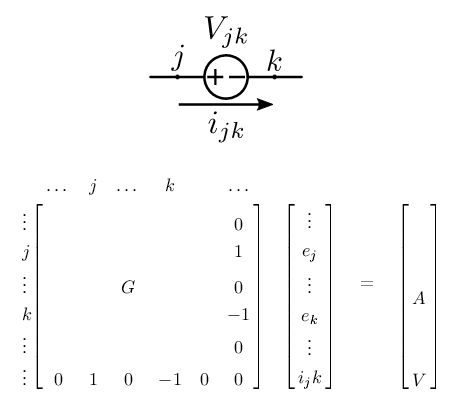
\includegraphics[scale=0.8]{img/IdealVoltageSource.png}
	\caption{ideal Voltage Source between nodes j and k}
	\label{fig:IdealVSource}
\end{figure}

\subsection{Other components}
Components such as capacitor, inductor and real voltage source (ideal voltage source in series with a resistance) can be represented by equivalent circuits, composed by a current source and a resistance. That means that the matrix stamp of these components is made by stamping a current source and a resistance on the matrix equation.

The method used to represent capacitors and inductors is detailed in section \ref{ResistiveCompanion}. The model used for a real voltage source is presented in subsection \ref{sub:RealVoltageSource}.

 
\section{Resistive Companion Method} \label{ResistiveCompanion}

\subsection{Inductor} \label{ResistiveCompanionInductor}
The presence of an inductor or a capacitor in a circuit introduces dynamics that require the knowledge of the "past" behavior of the component to represent its quantities at a given time.

An inductor can be described by the following equations: 

\begin{equation}
        v_L(t) = L \frac{di_L(t)}{dt}
\end{equation}

\begin{equation}
        i_L(t) = i_L(t- \Delta t) + \frac{1}{L} \cdot \int_{t- \Delta t}^{t} v_L(\tau) d \tau 
\end{equation}

In dynamic phasors the inductor equations become:

\begin{equation}
        v_L(t) = L \frac{di_L(t)}{dt} + j \omega \cdot L \cdot  i_L(t)
\end{equation}

\begin{equation}
        i_L(t) = i_L(t- \Delta t) +  \int_{t- \Delta t}^{t} \frac{1}{L} \cdot v_L(\tau) -j \omega \cdot i_L(\tau)d \tau 
\end{equation}

A numerical solution for these equations can only be obtained at a finite number of points, therefore a discretization of time is required.

For modeling inductors and capacitors, resistive companion method is used. Each dynamic component is transformed into a DC equivalent circuit, which represent one iteration of an integration method.
There are different integration methods available to solve the integration problem. The method chosen in this work is the trapezoidal rule.

Given the following equation, that defines the value of a variable $y$ at the point $k+1$.

\begin{equation}
	y(k+1) = y(k) + \int_{t_k}^{t_k+ \Delta t} x(\tau)d \tau
\end{equation}

With the trapezoidal rule $y(k+1)$ is calculated as following:

\begin{equation}
	y(k+1)=y(k)+ \frac{x(k)+x(k+1)}{2} \cdot \Delta t
\end{equation}

Applying trapezoidal rule for the inductor equation in dynamic phasor:
\begin{equation}
        i_L(k+1) = i_L(k) + \frac{\Delta t}{2} \left[ \frac{1}{L} \cdot v_L(k+1) - j \omega \cdot i_L(k+1) + \frac{1}{L} \cdot v(k) - j \omega \cdot i_L(k) \right]
\end{equation}

Defining:

\begin{align}
	a &= \frac{\Delta t}{2L} \\
	b &= \frac{\Delta t \omega}{2}
\end{align}
		
The equation can be rewritten as

\begin{align}
        i_L(k+1) &= i_L(k) + a \cdot v_L(k+1) - j b \cdot i_L(k+1) + a \cdot v(k) - j b \cdot i_L(k) \\
        i_L(k+1) &= \frac{1-b^2-j2b}{1+b^2}i_L(k) + \frac{a-jab}{1+b^2} v_L(k) + \frac{a-jab}{1+b^2} v_L(k+1)
\end{align}

The equation shows that the inductor current at the step k+1 has a part which depends on the voltage and current at the step k and a part which depends on the actual voltage. Therefore, the inductor can be substituted with a resistance $R_L$ in parallel with a current source $A_L(k)$. The value of $R_L$ is constant for a constant frequency and constant time step. The value of $A_L(k)$ depends on the knowledge of the previous step and has to be updated for each iteration.

\begin{figure}[ht]
	\centering
	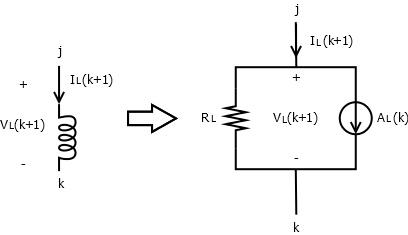
\includegraphics[scale=0.6]{img/Inductor.png} 
	\caption{Equivalent circuit of an Inductor}
	\label{fig:Inductor}
\end{figure}

 
\begin{equation} \label{eq:AL}
	A_L(k) = i_L(k) \cdot \frac{1-b^2-2bj}{1+b^2} + v_L(k) \cdot \frac{a-jab}{1+b^2}
\end{equation}

\begin{equation}
	R_L = \frac{1+b^2}{a-jab}
\end{equation}	

For an inductor connected between nodes j and k, the matrix stamp is made as following.

\begin{align}
\begin{split}
&
\begin{matrix}
& \cdots & j & \quad k & \cdots
\end{matrix}\\[-6pt]
\begin{matrix}
\vdots\\[6pt]
j\\[6pt]
k\\[6pt]
\vdots\\
\end{matrix}
&
\begin{bmatrix}
	\quad & \quad &  \\[6pt]
	\quad & \dfrac{1}{R_L} & \dfrac{-1}{R_L} & \quad  \\[6pt]
	\quad & \dfrac{-1}{R_L} & \dfrac{1}{R_L} & \quad \\[6pt]
	\quad &  & 
\end{bmatrix}
\begin{bmatrix}
	\quad \\[6pt]
	e_j(k+1)\\[6pt]
	e_k(k+1)\\[6pt]
	\quad
\end{bmatrix}
=
\begin{matrix}
\vdots\\[6pt]
j\\[6pt]
k\\[6pt]
\vdots\\
\end{matrix}
\begin{bmatrix}
	\quad \\[6pt]
	-A_L(k)\\[6pt]
	A_L(k)\\[6pt]
	\quad
\end{bmatrix}
\end{split}
\end{align}

\subsection{Capacitor} \label{ResistiveCompanionCapacitor}

The same approach used for the inductor is used now for the capacitor.
A capacitor can be described by the following equations:

\begin{equation}
	i_C(t)= C \frac{d v_c}{dt}
\end{equation}

\begin{equation}
	v_C(t)= v_C(t - \Delta t) + \frac{1}{C} \int_{t - \Delta t}^{t} i_C (\tau) d \tau
\end{equation}

In dynamic phasor the capacitor equations become:

\begin{equation}
        i_C(t)= C \frac{d v_c}{dt} + j \omega \cdot C \cdot v_C(t)
\end{equation}

\begin{equation}
        v_C(t) = v_C(t- \Delta t) +  \int_{t- \Delta t}^{t} \frac{1}{C} \cdot i_C(\tau) -j \omega \cdot v_C(\tau)d \tau 
\end{equation}

Applying trapezoidal rule for the capacitor equation:

\begin{equation}
        v_C(k+1) = v_C(k) + \frac{\Delta t}{2} \left[ \frac{1}{C} \cdot i_C(k+1) - j \omega \cdot v_C(k+1) + \frac{1}{C} \cdot i_C(k) - j \omega \cdot v_C(k) \right]
\end{equation}

Defining:
\begin{align}
        a &= \frac{\Delta t}{2C} \\
        b &= \frac{\Delta t \omega}{2}
\end{align}

\begin{align}
        v_C(k+1) &= v_C(k) + a \cdot i_C(k+1) - j b \cdot v_C(k+1) + a \cdot i_C(k) - j b \cdot v_C(k) \\
        i_C(k+1) &= \frac{1+jb}{a} \cdot v_C(k+1) - \frac{1-jb}{a} \cdot v_C(k) -i_C(k)
\end{align}

The capacitor in calculation step k+1 can also be substituted with a resistance $R_C$ in parallel with a current source $A_C(k)$.The value of $R_C$ is constant for a constant frequency and constant time step. The value of $A_C(k)$ depends only on the previous time step and changes for each iteration.

\begin{equation} \label{eq:AC}
	A_C = \frac{1-jb}{a} v_C(k) + i_C(k)
\end{equation}

\begin{equation}
	R_C = \frac{a}{1+jb}
\end{equation}

For a capacitor connected between nodes j and k, the matrix stamp is made as following:

\begin{align}
\begin{split}
&
\begin{matrix}
& \cdots & j & \quad k & \cdots
\end{matrix}\\[-6pt]
\begin{matrix}
\vdots\\[6pt]
j\\[6pt]
k\\[6pt]
\vdots\\
\end{matrix}
&
\begin{bmatrix}
	\quad & \quad &  \\[6pt]
	\quad & \dfrac{1}{R_C} & \dfrac{-1}{R_C} & \quad  \\[6pt]
	\quad & \dfrac{-1}{R_C} & \dfrac{1}{R_C} & \quad \\[6pt]
	\quad &  & 
\end{bmatrix}
\begin{bmatrix}
	\quad \\[6pt]
	e_j(k+1)\\[6pt]
	e_k(k+1)\\[6pt]
	\quad
\end{bmatrix}
=
\begin{matrix}
\vdots\\[6pt]
j\\[6pt]
k\\[6pt]
\vdots\\
\end{matrix}
\begin{bmatrix}
	\quad \\[6pt]
	A_C(k)\\[6pt]
	-A_C(k)\\[6pt]
	\quad
\end{bmatrix}
\end{split}
\end{align}

\begin{figure}[ht]
	\centering
	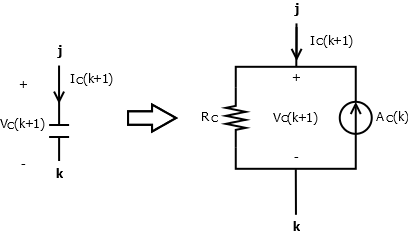
\includegraphics[scale=0.6]{img/Capacitor.png} 
	\caption{Equivalent circuit of a Capacitor}
	\label{fig:Capacitor}
\end{figure}



